\documentclass[10pt,twocolumn]{article}
\usepackage[margin=0.72in,columnsep=0.22in]{geometry}
\usepackage{times}
\usepackage{amsmath,amssymb}
\usepackage{booktabs}
\usepackage{graphicx}
\usepackage{microtype}
\usepackage{xcolor}
\usepackage{hyperref}
\hypersetup{colorlinks=true,linkcolor=blue!60!black,citecolor=blue!60!black,urlcolor=blue!60!black}

\title{\textbf{When Do Physiological Constraints Hurt Clinical Pretraining?}\\
\large Scale Dominance and Evaluation Pitfalls in Cross-Hospital Transfer}

\author{Anonymous Author(s) \\
\small Submission for AAAI Workshop Evaluation}
\date{}

\begin{document}
\maketitle

\begin{abstract}
Incorporating algebraic physiological laws into clinical masked pretraining promises stronger cross-hospital transfer. Across PhysioNet 2019 sepsis (\textbf{10,381} source and \textbf{14,779} target stays, \textbf{304} positives) and fixed-window ($T=48$) MIMIC-IV/eICU-CRD mortality (\textbf{122,611} stays), we audit physiology-constrained learning (PCL) against empirical risk minimization (ERM) under matched budgets and pre-registered controls. At default penalty weights ($\lambda \ge 0.5$), PCL never beats ERM: under matched $25\text{k}$-stay ($10{,}800$-step) pretraining, source-only fine-tuned PCL trails ERM on Site B sepsis ($\Delta = -0.0634$ AUROC, $p_t = 0.0052$, exact $p_{\mathrm{perm}} = 0.0625$, $p_{\mathrm{Holm}} = 0.375$), while per-seed source-validation tuning over $\lambda \in \{0.01,\dots,1\}$ picks small $\lambda \le 0.05$ ($0.679$ vs.\ $0.687$ ERM). Mechanistically, encoder task and constraint gradients are nearly orthogonal ($\cos \approx 0$), yet raw PCL gradient norms exceed masked reconstruction by $60\text{--}165\times$ for $\lambda \ge 0.5$---reproducing PINN gradient-scale dominance---while a channel-permuted \textit{Placebo} trails ERM ($0.663$ vs.\ $0.692$). Finally, tabular \texttt{HistGBM} baselines outperform $3.2\text{M}$ Transformers on $T=48$ mortality ($0.819$--$0.830$), underscoring optimization and architectural limits.
\end{abstract}

\section{Introduction}
Cross-hospital deployment of clinical time-series models often degrades under shifts in charting frequency, laboratory protocols, and patient case mix. A natural regularizer is \emph{physiology-constrained learning} (PCL): penalizing masked-reconstruction pretraining with residuals of differentiable physiological equations—mean arterial pressure conservation, pulse pressure, shock index, Henderson--Hasselbalch (HH) acid-base equilibrium, and Severinghaus $\text{SpO}_2$ kinetics—to discourage spurious hospital-specific features.

Although prior uncalibrated evaluations suggested gains from PCL, rigorous auditing uncovers serious confounds: unmatched optimization steps, post-discharge sequence padding, representation norm inflation, and severe cross-hospital differences in arterial blood gas (ABG) ordering. Crucially, multi-term constraint balancing mirrors well-known \emph{gradient-scale pathologies} in physics-informed neural networks (PINNs) \cite{wang2021understanding,krishnapriyan2021characterizing}. Rather than assuming physiological constraints fail universally, we test \emph{which penalty weights, optimization scales, and modeling assumptions} drive PCL's transfer behavior:
\begin{enumerate}
    \item \textbf{Controlled Budgets \& Placebo Controls:} Holding pretraining volume and steps equal ($10\text{k} \to 25\text{k} \to 80\text{k}$ resampled Site A stays), ERM matches or exceeds PCL across every budget ($0.753$ vs.\ $0.726$ at 80k), while a randomly permuted \textit{Placebo} constraint trails ERM ($0.663$ vs.\ $0.692$, $p_t = 0.0057$).
    \item \textbf{Gradient-Scale Dominance ($\cos \approx 0$):} Sweeping $\lambda \in \{0, 0.01, 0.05, 0.1, 0.5, 1.0\}$ shows PCL and masked-prediction encoder gradients are nearly orthogonal ($\cos \in [-0.023, +0.006]$), but effective PCL gradient norms dominate reconstruction by $60.2\times$ ($\lambda=0.5$) and $164.8\times$ ($\lambda=1.0$). Per-seed validation tuning selects $\lambda \le 0.05$, still failing to beat ERM ($0.679$ vs.\ $0.687$).
    \item \textbf{Evaluation Pitfalls \& Baselines:} We verify post-discharge length leakage in variable-window length of stay (LOS), document a $50.1\times$ drop in HH firing on Site B alongside derived-variable tautologies, run an exploratory \texttt{LayerNorm}/\texttt{LP-FT} head pilot \cite{kumar2022fine}, and benchmark against tabular \texttt{HistGBM} across tasks.
\end{enumerate}

\section{Cohorts, Architecture, and Protocol}

\paragraph{Pool Composition \& Cohort Accounting.}
Table~\ref{tab:cohort} details all four datasets (totaling $230{,}213$ ICU stays; per-cohort unique patient counts total $182{,}618$ without cross-dataset linkage). Pretraining uses $17$ physiological variables scaled with fixed clinical plausibility bounds (\texttt{MinMaxNormalizer}, zero split-derived statistics). Clean pretraining uses PhysioNet Site A ($10{,}381$ stays). Crucially, the \textbf{25k} and \textbf{80k} matched-volume controls bootstrap-resample \emph{Site A only} with replacement to match step counts ($10{,}800$ and $30{,}000$ steps); no MIMIC-IV or target Site B stays enter clean or matched-volume pretraining. Two explicit \textit{transductive} arms (\texttt{Target-Exposed 25k A+B}) resample unlabeled Site B stays without labels. Note that Site A and MIMIC-IV both originate from Beth Israel Deaconess Medical Center (BIDMC), reflecting EHR-era rather than health-system shift. On Site B sepsis evaluation ($14{,}779$ stays), true sepsis prevalence is $2.057\%$ ($304$ positives), giving constant-predictor baselines of $\mathrm{Brier} = 0.02015$ and $\mathrm{AUPRC} = 0.02057$. Fixed-$T=48$ mortality evaluation retains stays $\ge 48\text{h}$ ($46{,}158$ MIMIC-IV; $76{,}453$ eICU-CRD).

\begin{table}[t]
\centering
\caption{Reconciled per-cohort accounting across PhysioNet 2019 \cite{reyna2019early}, MIMIC-IV \cite{johnson2023mimic}, and eICU-CRD \cite{pollard2018eicu}. Mortality labels exist on MIMIC-IV/eICU-CRD; sepsis and LOS exist on PhysioNet.}
\label{tab:cohort}
\scriptsize
\begin{tabular}{lrrrrr}
\toprule
Cohort & Stays & Patients & LOS Mean & $<48$h & Mort. Prev. \\
\midrule
PhysioNet Site A & 10,381 & 10,381 & 46.2 h & 66.5\% & n/a \\
PhysioNet Site B & 14,779 & 14,779 & 45.3 h & 68.9\% & n/a \\
MIMIC-IV v3.1 & 74,607 & 54,427 & 105.4 h & 38.1\% & 11.89\% \\
eICU-CRD v2.0 & 130,446 & 103,031 & 90.4 h & 41.4\% & 9.10\% \\
\bottomrule
\end{tabular}
\end{table}

\paragraph{Backbone, Constraints \& Tuning Parity.}
All neural arms share a 6-layer Transformer ($d_{\mathrm{model}}=256$, $3.2\text{M}$ parameters) trained for $30$ FP32 epochs (mask probability $0.3$, AdamW, cosine decay, gradient clip norm $1.0$). PCL adds weighted physiological residuals (MAP weight $1.0$, HH $1.0$, $\text{SpO}_2$ $1.0$; PP and SI weighted $0$ by default) with an adaptive EMA loss balancer ($\mathrm{momentum}=0.95$). Both ERM and PCL use identical hyperparameter schedules during source-only fine-tuning ($30$ epochs: $10$ frozen-encoder, $20$ unfrozen with encoder LR $0.1\times$ head LR), selecting checkpoints on an 80/20 Site A validation split by validation AUROC (or validation $\log(1+\mathrm{LOS})$ MSE, evaluated back in hours). Notice matched step counts give PCL slightly higher FLOPs per step due to constraint evaluation, favoring PCL conservatively.

\paragraph{Statistical Protocol.}
We separate \textbf{Confirmatory} ($2\times 2$ volume $\times$ method) contrasts from \textbf{Exploratory} ablations ($n=5$ paired seeds: $42\text{--}46$). Because two-sided exact sign-flip permutation at $n=5$ ($2^5=32$ flips) has a minimum achievable $p$-value of $2/32 = 0.0625$, we report both paired $t$-tests and exact permutation $p$-values alongside \textbf{Holm--Bonferroni} family adjustments \cite{holm1979simple}, \textbf{TOST} equivalence tests \cite{lakens2017equivalence} at $\Delta \in \{0.01, 0.02\}$, and tie-safe \textbf{patient-level cluster bootstrap} ($B \in \{5{,}000, 10{,}000\}$) on Site B test predictions when saved. We never interpret $p > 0.05$ as equivalence unless TOST rejects non-equivalence.

\section{Results}

\subsection{Controlled Budgets, Placebo \& Ablations}

\begin{figure*}[t]
\centering
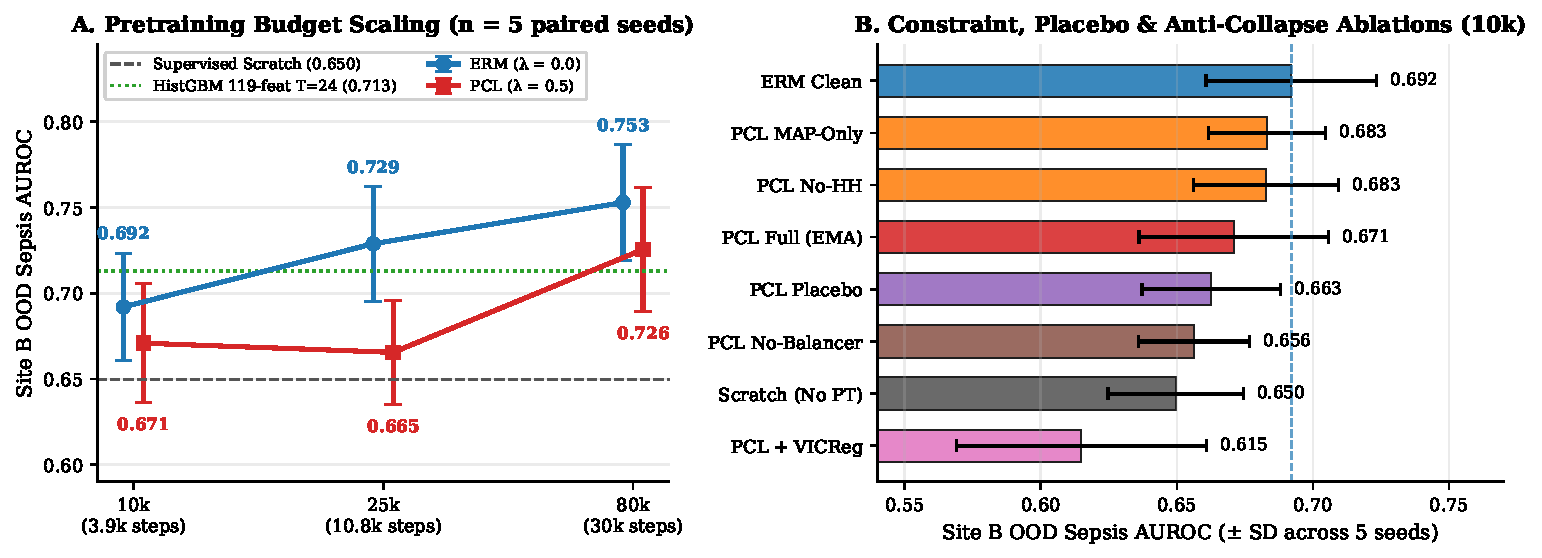
\includegraphics[width=\textwidth]{figures/fig1_budget_and_ablations.pdf}
\caption{\textbf{A.} Site B sepsis AUROC across equalized Site A pretraining budgets ($10\text{k} \to 25\text{k} \to 80\text{k}$ stays; $n=5$ seeds, $\pm$ SD). ERM climbs steadily to $0.753$, surpassing 119-feature \texttt{HistGBM} ($T=24$, $0.713$). \textbf{B.} 10k constraint, placebo, and VICReg ablations.}
\label{fig:fig1}
\end{figure*}

Table~\ref{tab:phase2c} and Figure~\ref{fig:fig1} summarize all controlled sepsis and fixed-$T=24$ LOS arms ($n=5$ seeds: $42\text{--}46$).

\begin{table*}[t]
\centering
\caption{Source-only fine-tuning on PhysioNet Site A $\to$ Site B across matched pretraining budgets, constraint ablations, and representation interventions ($n=5$ paired seeds $42\text{--}46$, mean $\pm$ SD; Site B prevalence $= 2.057\%$, constant AUPRC $= 0.0206$).}
\label{tab:phase2c}
\scriptsize
\begin{tabular}{lcccccc}
\toprule
Condition & Steps & $L_2$ Norm (h47) & Spread (h47) & Site B Sepsis AUROC & Site B AUPRC & LOS $T=24$ $R^2$ \\
\midrule
Supervised Scratch (Random Init) & 0 & --- & --- & $0.6495 \pm 0.0248$ & $0.1220 \pm 0.0125$ & $-0.0072 \pm 0.0129$ \\
ERM Clean (10k Site A) & 3.9k & $106.80 \pm 3.45$ & $0.2247 \pm 0.0063$ & $0.6920 \pm 0.0313$ & $0.1273 \pm 0.0265$ & --- \\
ERM Matched-Vol (25k Site A) & 10.8k & $73.74 \pm 3.71$ & $0.5350 \pm 0.0176$ & $0.7289 \pm 0.0336$ & $\mathbf{0.1506 \pm 0.0115}$ & $-0.0041 \pm 0.0078$ \\
ERM Target-Exposed (25k A+B) & 10.8k & $72.50 \pm 7.93$ & $0.5302 \pm 0.0546$ & $0.7269 \pm 0.0335$ & $0.1462 \pm 0.0259$ & --- \\
\textbf{ERM Matched-Vol (80k Site A)} & 30.0k & $\mathbf{59.80 \pm 4.12}$ & $\mathbf{0.8149 \pm 0.0331}$ & $\mathbf{0.7529 \pm 0.0337}$ & $0.1181 \pm 0.0244$ & $-0.0477 \pm 0.0384$ \\
\midrule
PCL Clean (10k, $\lambda=0.5$, EMA) & 3.9k & $164.11 \pm 5.89$ & $0.1098 \pm 0.0060$ & $0.6709 \pm 0.0348$ & $0.1223 \pm 0.0061$ & --- \\
PCL Clean (10k, $\lambda=1.0$, EMA) & 3.9k & --- & --- & $0.6600 \pm 0.0155$ & --- & --- \\
PCL Fixed-Weight (No Balancer) & 3.9k & $182.44 \pm 6.15$ & $0.1061 \pm 0.0034$ & $0.6562 \pm 0.0204$ & $0.0799 \pm 0.0397$ & $-0.0146 \pm 0.0251$ \\
PCL Matched-Vol (25k Site A) & 10.8k & $154.73 \pm 13.33$ & $0.2185 \pm 0.0171$ & $0.6655 \pm 0.0303$ & $0.1244 \pm 0.0146$ & $-0.0392 \pm 0.0526$ \\
PCL Target-Exposed (25k A+B) & 10.8k & $151.96 \pm 6.82$ & $0.2334 \pm 0.0128$ & $0.6808 \pm 0.0331$ & $0.1296 \pm 0.0170$ & --- \\
PCL Matched-Vol (80k Site A) & 30.0k & $289.35 \pm 54.11$ & $0.2832 \pm 0.0461$ & $0.7255 \pm 0.0362$ & $0.1497 \pm 0.0238$ & $-0.0249 \pm 0.0077$ \\
\midrule
PCL MAP-Only (10k, HH=0, SpO2=0) & 3.9k & $160.04 \pm 8.16$ & $0.1143 \pm 0.0051$ & $0.6831 \pm 0.0215$ & $0.1395 \pm 0.0228$ & $-0.0173 \pm 0.0191$ \\
PCL No-HH (10k, MAP+SpO2) & 3.9k & $160.76 \pm 3.49$ & $0.1126 \pm 0.0048$ & $0.6828 \pm 0.0267$ & $0.1417 \pm 0.0282$ & $-0.0026 \pm 0.0114$ \\
PCL Placebo (10k, Permuted) & 3.9k & $120.15 \pm 18.73$ & $0.1559 \pm 0.0859$ & $0.6627 \pm 0.0255$ & $0.1014 \pm 0.0225$ & $-0.0185 \pm 0.0081$ \\
PCL + VICReg (10k, \cite{bardes2022vicreg}) & 3.9k & $87.08 \pm 1.52$ & $0.0443 \pm 0.0015$ & $0.6149 \pm 0.0460$ & $0.0605 \pm 0.0434$ & $-0.0147 \pm 0.0184$ \\
\bottomrule
\end{tabular}
\end{table*}

\paragraph{Budget Scaling \& Statistical Contrasts.}
At $n=5$, resampling Site A ($10\text{k} \to 25\text{k}$) increases ERM ($\Delta = +0.0368$, $95\%$ CI $[+0.0006, +0.0730]$, $p_t = 0.0476$, $p_{\mathrm{perm}} = 0.0625$) while PCL remains flat ($\Delta = -0.0054, p_t = 0.8157$). At matched $25\text{k}$ volume, PCL trails ERM by $\Delta = -0.0634$ ($95\%$ CI $[-0.0952, -0.0315]$, $p_t = 0.0052$, exact $p_{\mathrm{perm}} = 0.0625$, $p_{\mathrm{Holm}} = 0.3750$ due to the $n=5$ floor). Equal-budget \textbf{ERM 80k} reaches $\mathbf{0.7529 \pm 0.0337}$ (Site B patient bootstrap $95\%$ CI $[0.7291, 0.7763]$; $+0.0608$ over ERM 10k, $p_t = 0.0212$), beating 119-feature \texttt{HistGBM} ($0.713 \pm 0.004$). Against ERM 80k, PCL 80k averages $-0.0274$ ($95\%$ CI $[-0.0913, +0.0365]$, $p_t = 0.3002$, $p_{\mathrm{perm}} = 0.3125$): not statistically distinguishable at $n=5$ (and TOST inconclusive against ERM 25k, $p=0.301$). Notably, ERM 80k exhibits higher AUROC yet lower uncalibrated raw AUPRC ($0.1181$ vs.\ $0.1506$ at 25k), consistent with high-threshold precision noise across $304$ positives ($2.06\%$ prevalence). Against Scratch ($0.6495$), ERM 10k ($+0.0425$, $p_t = 0.0109$) and ERM 25k ($+0.0793$, $p_t = 0.0058$) clearly help, whereas PCL 10k ($\lambda=0.5$: $+0.0214$, $p_t = 0.4243$; $\lambda=1.0$: $-0.0320$ vs.\ ERM 10k, $p_{\mathrm{perm}}=0.125$) shows no detectable benefit.

\paragraph{Physics Content vs.\ Penalty Scale \& Documentation Shift.}
Applying PCL's loss forms to \emph{randomly permuted channels} (\textit{Placebo}, $0.6627$) trails ERM 10k ($\Delta = -0.0294$, $p_t = 0.0057$, $p_{\mathrm{perm}} = 0.0625$), while remaining statistically indistinguishable from Full PCL ($\Delta = -0.0082$, $p_{\mathrm{perm}}=0.750$, TOST inconclusive $p=0.307$). Similarly, No-HH ($0.6828$) and MAP-Only ($0.6831$) sit $+0.012$ above Full PCL against an SD of $0.027$ ($p_t = 0.58$--$0.62$). Appendix Table~\ref{tab:abg} explains why: Site B experiences a $50.1\times$ drop in hourly HH firing ($24.2\% \to 0.48\%$ of hours; $2.23\%$ of stays), meaning HH is nearly inactive on the target—and clinically, ABG analyzers often calculate $\text{HCO}_3^-$ directly from $\text{pH}$ and $\text{PaCO}_2$, making HH an algebraic derived-variable tautology.

\subsection{\texorpdfstring{$\lambda$}{lambda} Sweep, Source-Val Tuning \& Gradient-Scale Dominance}

\begin{figure*}[t]
\centering
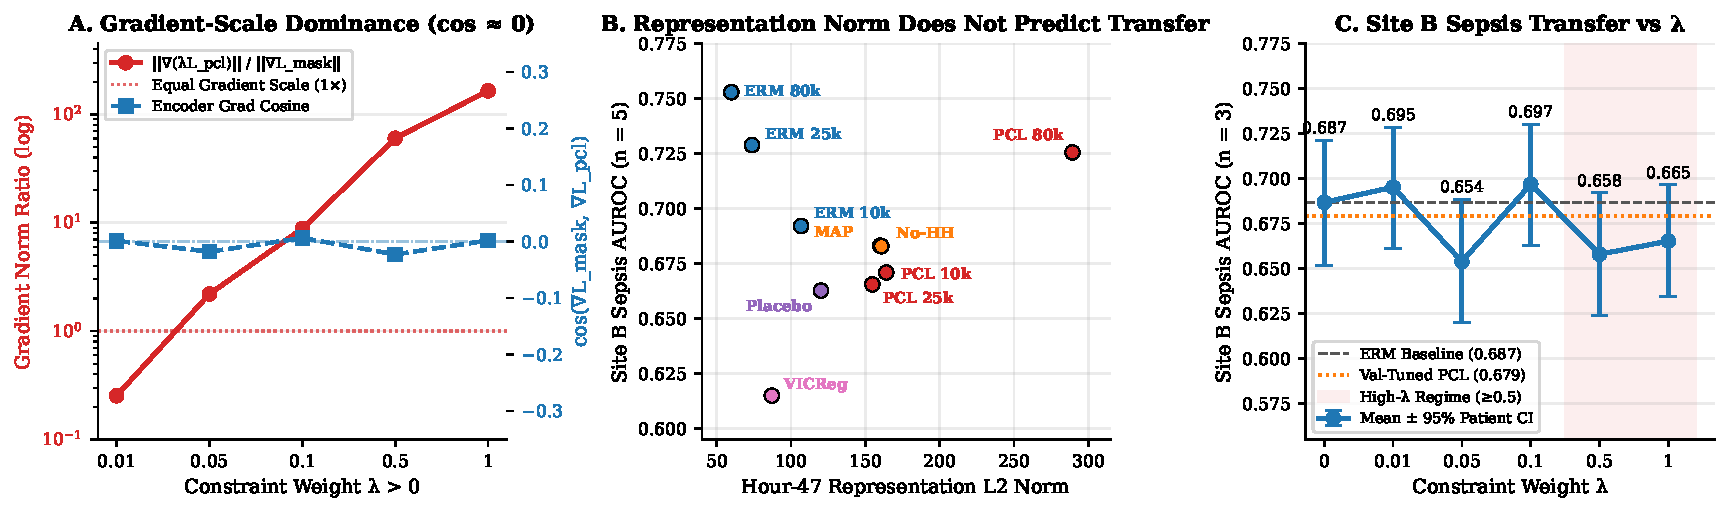
\includegraphics[width=\textwidth]{figures/fig2_lambda_dose_response.pdf}
\caption{\textbf{A.} Encoder gradient norms and cosine similarity across $\lambda \in \{0.01,\dots,1.0\}$ (15 batches across seeds $42\text{--}44$): gradients are orthogonal ($\cos \approx 0$), yet PCL's effective gradient norm dominates masked reconstruction up to $164.8\times$. \textbf{B.} Hour-47 representation $L_2$ norm vs.\ Site B AUROC across all Phase 2c arms shows norm does not explain transfer. \textbf{C.} Site B AUROC vs.\ $\lambda$ ($n=3$, $95\%$ patient bootstrap CIs; orange dotted line shows per-seed source-val $\lambda$ selection at $0.679$).}
\label{fig:fig2}
\end{figure*}

We swept $\lambda \in \{0, 0.01, 0.05, 0.1, 0.5, 1.0\}$ ($n=3$ seeds $42\text{--}44$; ERM $\lambda=0$ shares the same pretrained seed initialization as Table~\ref{tab:phase2c}, differing only across $n=3$ vs.\ $n=5$ fine-tunes) and measured pretraining gradient norms, weighted loss share, and encoder gradient cosine similarity $\cos(\nabla_\theta L_{\mathrm{masked}}, \nabla_\theta L_{\mathrm{pcl}})$ (Figure~\ref{fig:fig2}):
\begin{itemize}
    \item \textbf{Monotonic Loss Share, Orthogonal Gradients \& $165\times$ Scale Dominance:} By construction, average weighted PCL loss share rises strictly across $\lambda$-level means from $0.00\%$ ($\lambda=0$) $\to 0.82\%$ ($0.01$) $\to 4.44\%$ ($0.05$) $\to 8.22\%$ ($0.1$) $\to 30.06\%$ ($0.5$) $\to 44.72\%$ ($1.0$) ($\rho_{\mathrm{means}} = 1.000$ across the 6 levels). However, pretraining gradient norms jump $384\times$ ($0.0689 \to 26.43$, saturating the $1.0$ clip threshold at $\lambda \ge 0.1$). Crucially, measuring encoder gradient cosines directly shows $\cos \in [-0.023, +0.006]$ for $\lambda > 0$ (orthogonal, vs.\ $+0.264$ at $\lambda=0$), whereas the effective gradient-norm ratio $\|\nabla(\lambda L_{\mathrm{pcl,bal}})\| / \|\nabla L_{\mathrm{masked}}\|$ grows $0.25\times$ ($0.01$) $\to 2.20\times$ ($0.05$) $\to 8.81\times$ ($0.1$) $\to 60.16\times$ ($0.5$) $\to 164.75\times$ ($1.0$). Rather than opposing-direction conflict requiring gradient surgery \cite{yu2020gradient}, PCL suffers \emph{PINN-style gradient-scale dominance} \cite{wang2021understanding,krishnapriyan2021characterizing}.
    \item \textbf{Norm Does Not Explain Transfer:} Although representation $L_2$ norm grows with $\lambda$ ($106.8 \to 169.3$), Figure~\ref{fig:fig2}B disproves norm inflation as the causal bottleneck: VICReg lowers norm ($87.1$) yet collapses transfer ($0.615$), while PCL 80k has norm $289.4$ yet achieves $0.726$.
    \item \textbf{High $\lambda$ Hurts; Tuning $\lambda$ Still Fails to Beat ERM:} Site B patient bootstrap ($B=5{,}000$) shows $\lambda=0.01$ ($0.6952$, $p_{\mathrm{boot}}=0.051$) and $\lambda=0.1$ ($0.6968$, $p_{\mathrm{boot}}=0.093$) stay statistically indistinguishable from ERM ($0.6868$), whereas $\lambda \ge 0.5$ degrades significantly ($0.6579$ at $0.5$, $p_{\mathrm{boot}}<0.001$; $0.6652$ at $1.0$, $p_{\mathrm{boot}}=0.024$). Most importantly, choosing PCL's best $\lambda \in \{0.01,\dots,1\}$ per seed via Site A validation selects $\lambda=0.01$ (seed 42) and $\lambda=0.05$ (seeds 43, 44), averaging $\mathbf{0.6792 \pm 0.0476}$ vs.\ ERM's $\mathbf{0.6868 \pm 0.0322}$.
\end{itemize}

\subsection{Exploratory Head Pilot, Mortality Ceiling \& LOS Audit}

\begin{figure*}[t]
\centering
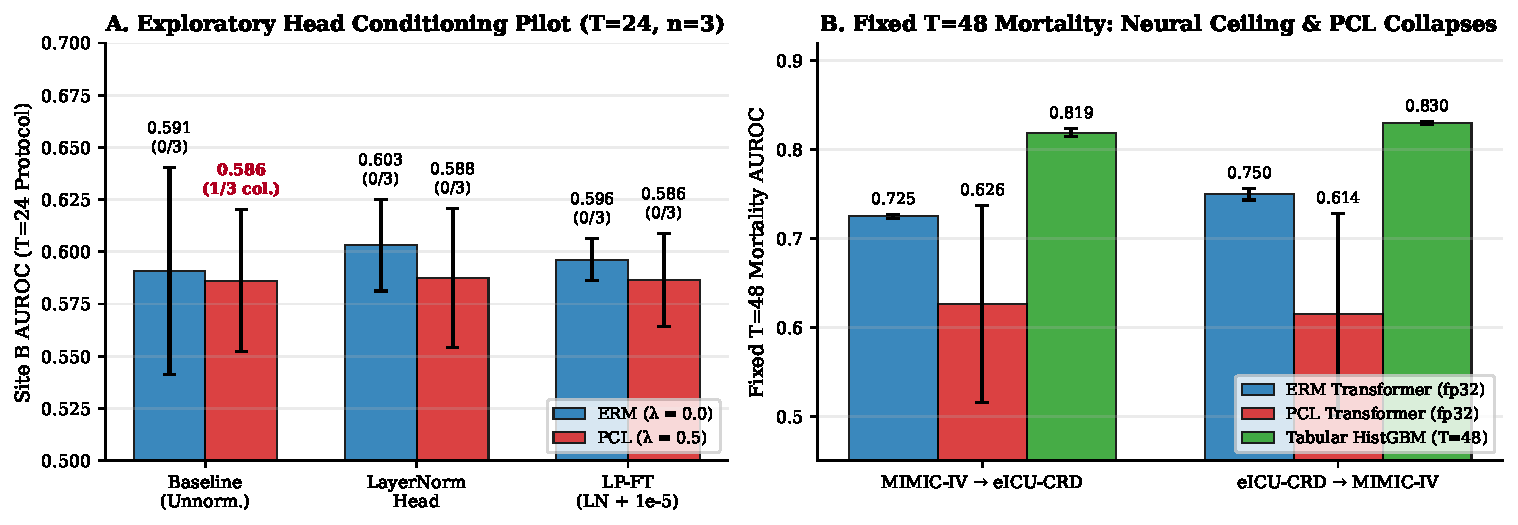
\includegraphics[width=\textwidth]{figures/fig3_head_pilot_and_tasks.pdf}
\caption{\textbf{A.} Exploratory head conditioning pilot on $T=24$ Sepsis ($n=3$): \texttt{LayerNorm}/\texttt{LP-FT} avoids PCL's $1/3$ collapse warning but sits in a low-signal $T=24$ regime ($\sim 0.59$). \textbf{B.} Fixed-$T=48$ Mortality (MIMIC-IV $\leftrightarrow$ eICU-CRD): PCL experiences $1/3$ collapses at $0.500$ ($0.626$/$0.614$) while tabular \texttt{HistGBM} reaches $0.819$--$0.830$.}
\label{fig:fig3}
\end{figure*}

To test whether classification-head saturation explains PCL's fragility, we ran an exploratory pilot ($T=24$ Sepsis, $n=3$) comparing baseline, \texttt{LayerNorm}, and \texttt{LP-FT} \cite{kumar2022fine} (Figure~\ref{fig:fig3}A). Baseline PCL triggered $1/3$ constant-logit warnings ($0.586 \pm 0.034$), whereas \texttt{LayerNorm} ($0.588 \pm 0.033$) and \texttt{LP-FT} ($0.586 \pm 0.022$) had $0/3$ warnings. However, because truncating sepsis stays at $T=24$ drops late-stay signal and compresses all arms near $0.59$--$0.60$ (ERM $0.591$--$0.603$), this small-$n$ pilot cannot verify full-horizon rescue.

On fixed-$T=48$ bidirectional \textbf{Mortality} \cite{harutyunyan2019multitask} (Figure~\ref{fig:fig3}B), FP32 ERM achieves $0.7250 \pm 0.0022$ (MIMIC$\to$eICU) and $0.7497 \pm 0.0065$ (eICU$\to$MIMIC, $0/6$ collapses), whereas FP32 PCL ($\lambda=0.5$) drops to $0.6262 \pm 0.1109$ (MIMIC$\to$eICU, $1/3$ collapse at $0.499$) and $0.6145 \pm 0.1140$ (eICU$\to$MIMIC, $1/3$ at $0.500$). Crucially, tabular \texttt{HistGBM} on identical $T=48$ summary features reaches $0.8631$/$0.8573$ in-domain and $0.8192$/$0.8303$ OOD, exposing a large architectural ceiling in the $3.2\text{M}$ Transformer. On \textbf{LOS}, variable-window transfer ($R^2 = +0.229$ on Site B) is fully reproduced by a stay-length-only probe ($R^2 = +0.2289$, mask+length $+0.2164$), while restricting to fixed $T=24\text{h}$ (all stays $\ge 24\text{h}$, $0\%$ dropped, zero padding) collapses \emph{both} Transformers (Table~\ref{tab:phase2c}) and \texttt{HistGBM} ($+0.034$ Site A, $-0.037$ Site B) near zero—confirming that short-window first-24h signals lack cross-site LOS predictability.

\section{Limitations and Conclusion}
Three limitations remain for full-journal extension: (1) under PhysioNet DUA constraints, the \texttt{LayerNorm}/\texttt{LP-FT} pilot ran on public $T=24$ Sepsis rather than credentialed MIMIC-IV/eICU mortality, where head-conditioned runs across $\ge 5$ seeds are still needed to separate collapse rate from mean AUROC; (2) confirmatory $n=5$ contrasts face a $0.0625$ permutation floor ($p_{\mathrm{Holm}}=0.375$), requiring $n=10$ seeds for confirmatory family significance; and (3) gradient-normalized balancing (e.g., GradNorm / PCGrad) has not yet been tested as a positive fix. Overall, our results show that naive PCL regularizers act via gradient-scale dominance at high $\lambda$ ($\ge 0.5$) without encoding transferable clinical invariance—making strict fixed windows, matched budgets, placebo controls, and source-val $\lambda$ tuning essential before deploying constraint-regularized clinical models.

\bibliographystyle{plain}
\begin{thebibliography}{11}
\scriptsize
\bibitem{wang2021understanding} S. Wang, Y. Teng, and P. Perdikaris. Understanding and mitigating gradient flow pathologies in physics-informed neural networks. \emph{SIAM J. Sci. Comput.}, 43(5), 2021.
\bibitem{krishnapriyan2021characterizing} A. Krishnapriyan, A. Gholami, S. Zhe, R. Kirby, and M. W. Mahoney. Characterizing possible failure modes in physics-informed neural networks. \emph{NeurIPS}, 2021.
\bibitem{yu2020gradient} T. Yu, S. Kumar, A. Gupta, S. Levine, K. Hausman, and C. Finn. Gradient surgery for multi-task learning. \emph{NeurIPS}, 2020.
\bibitem{kumar2022fine} A. Kumar, A. Raghunathan, R. Jones, T. Ma, and P. Liang. Fine-tuning can distort pretrained features and underperform out-of-distribution. \emph{ICLR}, 2022.
\bibitem{bardes2022vicreg} A. Bardes, J. Ponce, and Y. LeCun. VICReg: Variance-invariance-covariance regularization for self-supervised learning. \emph{ICLR}, 2022.
\bibitem{lakens2017equivalence} D. Lakens. Equivalence tests: A practical primer for t tests, correlations, and meta-analyses. \emph{Soc. Psychol. Personal. Sci.}, 8(4):355--362, 2017.
\bibitem{holm1979simple} S. Holm. A simple sequentially rejective multiple test procedure. \emph{Scand. J. Statist.}, 6(2):65--70, 1979.
\bibitem{reyna2019early} M. A. Reyna et al. Early prediction of sepsis from clinical data: The PhysioNet/Computing in Cardiology Challenge 2019. \emph{CinC}, 2019.
\bibitem{johnson2023mimic} A. E. W. Johnson et al. MIMIC-IV, a freely accessible electronic health record dataset. \emph{Scientific Data}, 10(1):1, 2023.
\bibitem{pollard2018eicu} T. J. Pollard et al. The eICU Collaborative Research Database, a freely available multi-center database. \emph{Scientific Data}, 5:180178, 2018.
\bibitem{harutyunyan2019multitask} H. Harutyunyan, H. Khachatrian, D. C. Kale, G. Ver Steeg, and A. Galstyan. Multitask learning and benchmarking with clinical time series data. \emph{Scientific Data}, 6:96, 2019.
\end{thebibliography}

\appendix
\section{Constraint Firing \& ABG Documentation Shift}
\begin{table}[ht]
\centering
\caption{Empirical constraint mask firing rates across PhysioNet Site A ($10{,}381$ stays, $498{,}288$h) and Site B ($14{,}779$ stays, $709{,}392$h).}
\label{tab:abg}
\scriptsize
\begin{tabular}{lcccc}
\toprule
Constraint & Site A Hourly & Site B Hourly & Site B Stays & A$\to$B Shift \\
\midrule
MAP / PP & 77.2\% & 88.6\% & 100.0\% & $1.15\times$ up \\
Shock Index (SI) & 85.3\% & 89.5\% & 100.0\% & $1.05\times$ up \\
HH (Acid-Base) & \textbf{24.2\%} & \textbf{0.48\%} & \textbf{2.23\%} & \textbf{50.1$\times$ drop} \\
Severinghaus ($\text{SpO}_2$) & 22.9\% & 7.59\% & 28.1\% & $3.0\times$ drop \\
\bottomrule
\end{tabular}
\end{table}

\end{document}
